\documentclass[tikz,border=8pt]{standalone}
\usepackage[T1]{fontenc}
\usepackage{lmodern}
\usetikzlibrary{arrows.meta,positioning,shapes.geometric}
\definecolor{navy}{HTML}{0B3954}
\definecolor{blue}{HTML}{087E8B}
\definecolor{gold}{HTML}{F4B942}
\definecolor{paper}{HTML}{F7F9FB}
\begin{document}
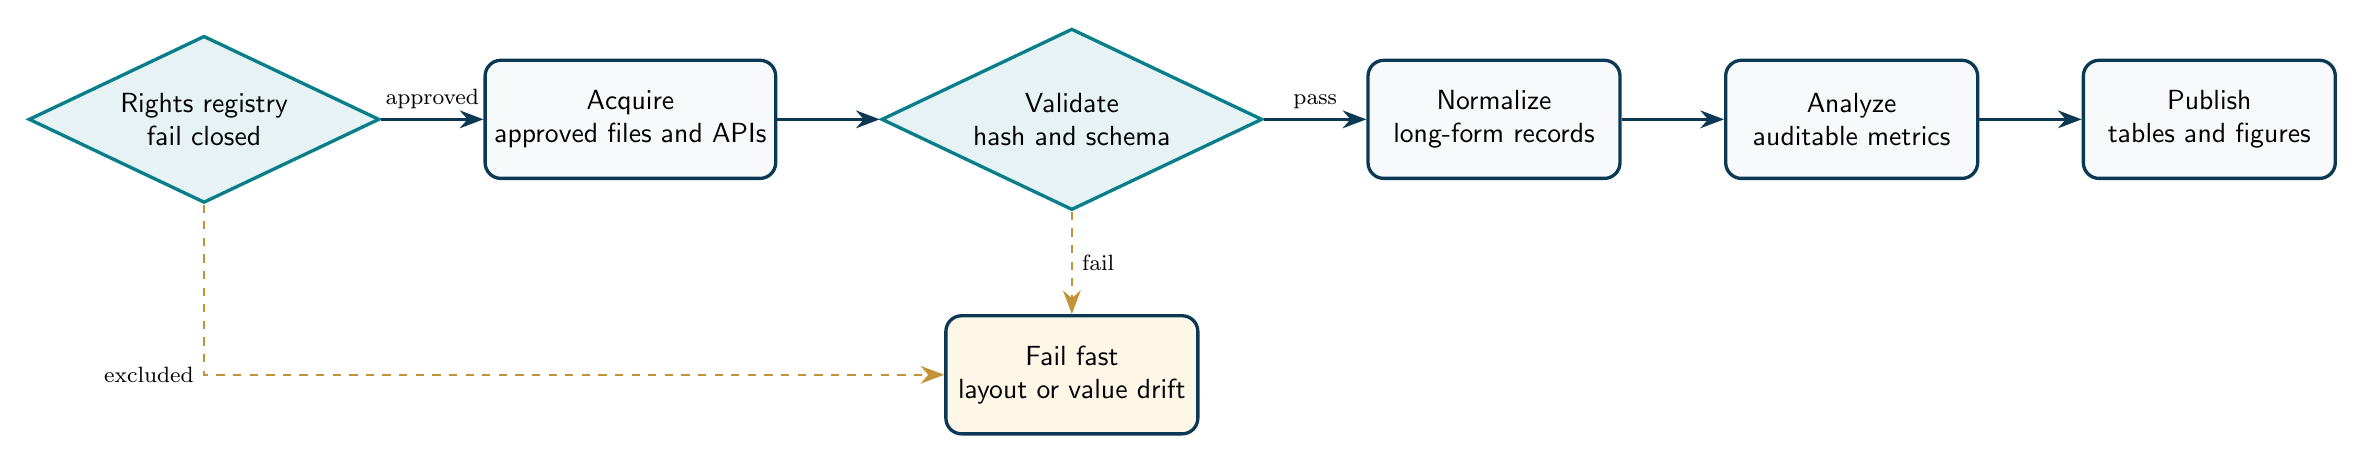
\begin{tikzpicture}[
  font=\sffamily,
  node distance=13mm,
  stage/.style={draw=navy, very thick, rounded corners=2mm, fill=paper,
    minimum width=32mm, minimum height=15mm, align=center},
  gate/.style={diamond, draw=blue, very thick, fill=blue!10,
    aspect=2.1, align=center, inner sep=1.5mm},
  flow/.style={-{Stealth[length=3mm]}, very thick, draw=navy},
  fail/.style={-{Stealth[length=3mm]}, thick, dashed, draw=gold!80!black}
]
\node[gate] (rights) {Rights registry\\fail closed};
\node[stage, right=of rights] (acquire) {Acquire\\approved files and APIs};
\node[gate, right=of acquire] (validate) {Validate\\hash and schema};
\node[stage, right=of validate] (normalize) {Normalize\\long-form records};
\node[stage, right=of normalize] (analyze) {Analyze\\auditable metrics};
\node[stage, right=of analyze] (publish) {Publish\\tables and figures};
\node[stage, below=of validate, fill=gold!12] (stop) {Fail fast\\layout or value drift};
\draw[flow] (rights) -- node[above, font=\footnotesize]{approved} (acquire);
\draw[flow] (acquire) -- (validate);
\draw[flow] (validate) -- node[above, font=\footnotesize]{pass} (normalize);
\draw[flow] (normalize) -- (analyze);
\draw[flow] (analyze) -- (publish);
\draw[fail] (rights) |- node[left, font=\footnotesize]{excluded} (stop);
\draw[fail] (validate) -- node[right, font=\footnotesize]{fail} (stop);
\end{tikzpicture}
\end{document}
